\documentclass[11pt]{article}

% Common packages
\usepackage{amsmath}   % advanced math environments
\usepackage{amssymb}   % math symbols
\usepackage{amsthm}    % theorem/proof environments (optional, kept for later)
\usepackage{geometry}  % page margins
\usepackage{enumitem}  % better lists
\usepackage{graphicx}  % include images
\usepackage{titlesec}
\usepackage{hyperref}  % hyperlinks (keep this LAST)
\usepackage{tikz}
\usetikzlibrary{trees}
\usepackage{pgfplots}
\usetikzlibrary{arrows.meta,positioning}
\pgfplotsset{compat=1.18}

% Page setup
\geometry{margin=0.5in}
\setlist[itemize]{topsep=2pt,itemsep=2pt,parsep=0pt}

% Short labels
\newcommand{\thm}{\underline{\textbf{Thm.}} }
\newcommand{\defn}{\underline{\textbf{Def.}} }
\newcommand{\prop}{\underline{\textbf{Prop.}} }
\DeclareMathOperator*{\argmax}{arg\,max}


% Title info
\title{ECON 4310 HW5}
\author{Michael Lee}

\begin{document}
\maketitle

\begin{enumerate}[label=\textbf{(\arabic*)}, leftmargin=*]
    \item \textbf{Overconfidence.} 
    \begin{enumerate}[label=\textbf{(\alph*)}, leftmargin=*]
            \item \textbf{\textit{Overall, what percentage of the workforce passes the evaluation?}}
            \[
            P(\text{Pass})
            = \frac{1}{3} \cdot \frac{19}{20} + \frac{1}{3} \cdot \frac{7}{16} + \frac{1}{3} \cdot \frac{33}{80}
            = 0.6
            \]

            \item \textbf{\textit{If a worker passes the evaluation, what is the probability they are in the top third?}}
            
            \[
            P(\text{Top Third} | \text{Pass})
            = \frac{P(\text{Pass} | \text{Top Third}) \cdot P(\text{Top Third})}{P(\text{Pass})}
            = \frac{1/3 \cdot 19/20}{0.6}
            = \frac{19}{36}
            \approx 0.5278
            \]

            \item \textbf{\textit{Suppose management decides to give the bonus to an employee if he or she believes they
            are more than 50\% likely to be in the top third. First, assuming employees take this
            as a true signal and are updating rationally, what percentage of the workforce gets the
            bonus?}} \\

            The firm gives the bonus to anyone who \textit{believes} they are more than 50\% likely to be in the top third. Thus, we need to find the probability that an employee believes they are in the top third. \\

            \(P(\text{Top Third} | \text{Pass}) = \frac{19}{36} \approx 0.5278\ > 0.5 \Rightarrow\) all passers believe they are more than 50\% likely to be in the top third, so they all qualify for the bonus. Thus, \(60 \%\) of the workforce gets the bonus. \\

            \item \textbf{\textit{Why might employees continue to believe they are more than 50\% likely to be in the
            top third even if they fail this test? (hint: this is not based on math)}} \\

            This is due to overconfidence. People systematically overestimate their own abilities and knowledge, leading them to believe they are more likely to be in the top third even if they fail the test. \\ 
    \end{enumerate}

    \item \textbf{Grim Trigger in the Repeated Prisoner's Dilemma.}
    \begin{enumerate}[label=\textbf{(\alph*)}, leftmargin=*]
        \item \textbf{\textit{Suppose that player 1 and player 2 are both following the grim trigger strategy. What
        actions will be played in each stage of the repeated game? What are the payoffs to
        players 1 and 2 in each stage?}}

        Let \(U_i(s_1, s_2)\) be the payoff to player \(i\) given player 1 uses strategy \(s_1\) and player 2 uses strategy \(s_2\). \\

        If both players follow the Grim Trigger Strategy (GT), they will both cooperate as neither has defected yet. Since neither defected in the first round, they will continue to cooperate in the next round. This process will repeat until the game stops. \\

        Thus, in each stage, their payoffs will be:
        \[
        (b-c, \, b-c)
        \]
        
        \item \textbf{\textit{Using your result from part 2a, write down the expected payoff to player 1 from the
        entire repeated prisoner's dilemma in terms of \(c\), \(b\), and \(\delta\).}}

        \[
        U_1(\text{GT}, \text{GT}) = (b-c) \delta(b-c) + \delta^2(b-c) + \cdots = \frac{b-c}{1-\delta}
        \]
        
        \item \textbf{\textit{Now we will check whether player 1 can improve his payoff by deviating from the grim
        trigger strategy. Here, we only need to check the case where player 1 plays all-D, that
        is, player 1 defects in every round. (This is because if player 1 deviates, then he must
        defect in some round. If he has incentive to defect in some round k, then by symmetry,
        player 1 has incentive to defect in the first round. But if player 1 defects in the first
        round, then player 2 defects forever, so it could not possibly be Nash for player 1 to
        cooperate in any round k.) What is the total payoff to player 1 from the entire repeated
        prisoner's dilemma if he deviates to all-D and player 2 continues to play grim trigger?}}

        Suppose player 1 deviates to all-D in the first round and player 2 continues using GT. Thus, in the first round, player 1 will play \(D\) and player 2 will play \(C\). However, in all subsequent rounds, both players will play \(D\). As a result, player 1's total payoff will be:
        \[
        U_1(\text{all-D}, \text{GT}) = (b) + (\delta \cdot 0) + (\delta^2 \cdot 0) + \cdots = b
        \]
        
        \item \textbf{\textit{For grim trigger to be a Nash equilibrium, we need that the payoff to player 1 from
        playing grim trigger is greater than or equal to the payoff to player 1 from playing all-D,
        assuming player 2's strategy is fixed. Using your results from parts 2b and 2c, write down
        an inequality that must be satisfied in order for grim trigger to be a Nash equilibrium.
        Simplify this inequality to obtain the condition \(\delta \geq \frac{c}{b}\).}}
        \[
        U_1(\text{GT}, \text{GT})
        = \frac{b-c}{1-\delta}
        \geq U_1(\text{all-D}, \text{GT})
        = b
        \Rightarrow
        b - c \geq (1-\delta)b
        \Rightarrow
        c \leq (1- \delta - 1)b
        \Rightarrow
        \delta \geq \frac{c}{b}
        \]

        \item \textbf{\textit{Interpret the comparative statics on this condition. Is this condition more or less likely
        to hold when \(\delta\), \(c\), or \(b\) increase?}}

        A higher \(\delta\) means that the chance of another round is higher. Thus, the threat of losing future cooperation becomes more powerful, making the inequality easier to satisfy and cooperation more likely. \\

        A higher \(c\) means that the cost of cooperation is higher, making defection more attractive. Thus, the people are less likely to cooperate, so the condition \(\delta \geq \frac{c}{b}\) is harder to hold. \\

        A higher \(b\) means that the benefit of cooperation is higher, making it more attractive. Thus, the people are more likely to cooperate, so the condition \(\delta \geq \frac{c}{b}\) is easier to hold. \\

        \item \textbf{\textit{In the class experiment where we played a dictator game after you earned points via
        a quiz, we saw giving decrease compared to the baseline dictator game (in terms of
        percentage given). How could this effect be interpreted through the lens of the condition
        found above?}} \\

        The results from our class dictator-game experiment align naturally with the inequality 
        \(\delta \ge \frac{c}{b}\). When participants had to give away earned quiz points rather
        than unearned money, they gave a noticeably smaller percentage. This suggests that the
        psychological and economic cost of giving, \(c\), felt higher (losing something you worked for
        is more painful than giving away windfall income). At the same time, the perceived social
        benefit of giving, \(b\), likely did not increase and may even have felt smaller because the
        money was tied to personal effort. Both effects raise the ratio \(c/b\), making the inequality
        harder to satisfy and cooperation (i.e., giving) less likely.

        \item \textbf{\textit{Continuing with the grim trigger strategy, we now ask: Is this equilibrium subgame
        perfect? Please explain why or why not. That is, suppose the players somehow arrive
        at a subgame in which Player 1 defected in the last round. Would Player 2 prefer to
        cooperate or defect in this round?}} \\

        If the players arrived at a subgame in which Player 1 defected in the last round, Player 2 would prefer to defect in this round. This is because Player 1 has already defected, so Player 2 will not get any future cooperation from Player 1. Thus, Player 2 will defect in this round to maximize their payoff.
    \end{enumerate}

    \item \textbf{More practice with subgame perfection}
    \begin{enumerate}[label=\textbf{(\alph*)}, leftmargin=*]
        \item \textbf{\textit{Imagine two coworkers are each deciding where to attend a weekend conference ---
        Chicago or San Francisco. They get extra utility \(c > 0\) for attending the same conference (they like to collaborate). But Alex prefers San Francisco and Jordan prefers
        Chicago (they each get \(b > 0\) from being in the city they enjoy). Assume they get \(0\)
        utility from being in the city they like least without the other. What is the condition
        such that (Chicago, Chicago) and (San Francisco, San Francisco) are both pure Nash
        Equilibria of the game?
        }} \\

        Let \(U_i(s_A, s_J)\) be the payoff to player \(i\) when Alex plays \(s_A\) and Jordan plays \(s_J\).

        Suppose Alex plays Chicago (CHI). Jordan could play either CHI or San Francisco (SF). However, Alex should play CHI:
        \[
        U_J(\text{CHI}, \text{SF}) = 0 < U_J(\text{CHI}, \text{CHI}) = b+c
        \]
        However, if Alex plays SF, Jordan could play either CHI or SF:
        \[
        U_J(\text{SF}, \text{CHI}) = b \quad \text{and} \quad U_J(\text{SF}, \text{SF}) = c
        \]
        In order for Jordan to prefer SF or be indifferent between the two options, \(c > b\).

        A similar argument can be made for Alex if Jordan plays SF or CHI. If Jordan plays SF, 
        \[
        U_A(\text{CHI}, \text{SF}) = 0 < U_A(\text{SF}, \text{SF}) = b + c
        \]
        If Jordan plays CHI,
        \[
        U_A(\text{CHI}, \text{CHI}) = c \quad \text{and} \quad U_A(\text{SF}, \text{CHI}) = b
        \]
        In order for Alex to prefer CHI or be indifferent between the two options, \(c > b\). \\

        Thus, in order for (CHI, CHI) and (SF, SF) to be both pure Nash equilibria, \(c > b > 0\).
        
        \newpage

        \item \textbf{\textit{Instead of simultaneous play, imagine that Jordan decides first on Thursday and Alex
        chooses after seeing Jordan's choice. Represent this now as a decision tree and solve for
        the subgame perfect Nash Equilibrium, assuming the condition you found in 3a}}. \\

        Let \(U(s_J, s_A) = (U_J, U_A)\) be the payoff for Jordan and Alex when Jordan plays \(s_J\) and Alex plays \(s_A\).

        \begin{figure}[h]
            \centering
            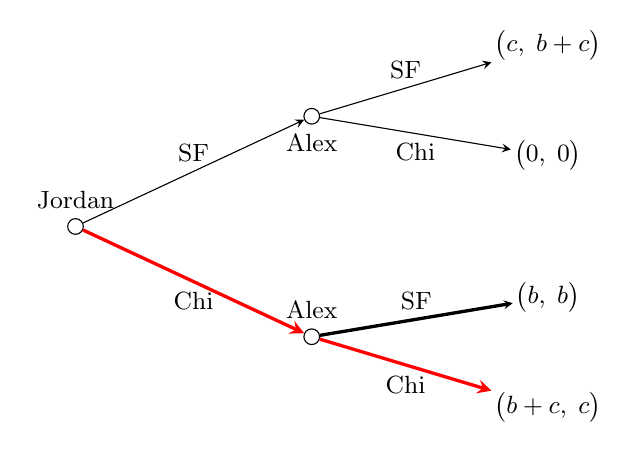
\begin{tikzpicture}[
              grow=right,
              level distance=30mm,
              level 1/.style={sibling distance=28mm},
              level 2/.style={sibling distance=18mm},
              every node/.style={font=\small},
              edge from parent/.style={draw, -stealth}
            ]
            
            % Root: Jordan
            \node[circle,draw,inner sep=2pt,label=above:{Jordan}] (J) {}
              % Jordan chooses Chicago (top branch) --- SPNE path (red)
              child {
                node[circle,draw,inner sep=2pt,label=above:{Alex}] (A1) {}
                  % Alex chooses Chi after Chi --- SPNE path (red)
                  child {
                    node[inner sep=1pt] {$\bigl(b+c,\;c\bigr)$}
                    edge from parent[draw=red, very thick, -stealth]
                      node[midway,below]{Chi}
                  }
                  % Alex chooses SF after Chi (off-path, force black)
                  child {
                    node[inner sep=1pt, yshift=-4mm] {$\bigl(b,\;b\bigr)$}
                    edge from parent[draw=black, -stealth]
                      node[midway,above]{SF}
                  }
                edge from parent[draw=red, very thick, -stealth]
                  node[midway,below]{Chi}
              }
              % Jordan chooses SF (bottom branch) (off-path, default black)
              child {
                node[circle,draw,inner sep=2pt,label=below:{Alex}] (A2) {}
                  child {
                    node[inner sep=1pt, yshift=4mm] {$\bigl(0,\;0\bigr)$}
                    edge from parent node[midway,below]{Chi}
                  }
                  child {
                    node[inner sep=1pt] {$\bigl(c,\;b+c\bigr)$}
                    edge from parent node[midway,above]{SF}
                  }
                edge from parent node[midway,above]{SF}
              };
            
            \end{tikzpicture}
            \caption{Extensive-form representation of the conference game (Jordan moves first). 
            The red path indicates the subgame perfect Nash equilibrium when $c > b > 0$.}
        \end{figure}
            
            
            
            
        

        \item \textbf{\textit{What does Jordan choose to do? Does the first or second mover in this game have the advantage?}} \\
        
        Alex will always choose whatever Jordan chooses, so Jordan should pick whatever maximizes their payoff. Since \(\argmax_{s_J} \{U_J(s_J, s_A)\} = \text{CHI}\) if \(c > b > 0\), Jordan should choose CHI. \\

        In this game, the first mover has the advantage as the second mover always prefers to make the same choice as the first mover.
    \end{enumerate}

    \item \textbf{Social Norms.}
    \begin{enumerate}[label=\textbf{(\alph*)}, leftmargin=*]
        \item \textbf{\textit{What is the behavior you are focused on? Briefly explain why you think increasing or
        decreasing this behavior would improve social welfare.}}

        As an RA, the behavior I focus on is students bringing up roommate problems to their RA. This behavior clearly affects social welfare
        because unresolved roommate issues can escalate into stress, sleep disruption, mental health concerns, academic decline, and
        broader floor-level tension. When residents proactively communicate problems to their RA, issues can usually be resolved
        early through mediation, room agreements, housing accommodations, or wellness referrals before they become severe. However,
        the student making the report often bears a private cost (awkwardness, fear of judgment, fear of retaliation, or feeling like
        they are “making things a big deal”), while the benefits are shared by both roommates and sometimes the entire community. This
        mismatch means the behavior is under-supplied relative to what would be socially optimal.

        \item \textbf{\textit{How can you measure what is motivating behavior? (e.g., how can you measure behaviors
        and beliefs in an incentive-compatible way to determine if this is a custom, moral rule,
        descriptive norm or social norm.)}}

        Because I am an RA, I can directly observe how residents behave, but to measure motivations more systematically I would pair
        behavioral measures with incentivized belief elicitation.

        \begin{enumerate}
            \item \textbf{Behavioral Measures:} In a short, anonymous questionnaire, I would give residents realistic scenarios (e.g. “Your roommate repeatedly violates quiet hours,” “Your roommate brings guests over without asking”) and ask whether they would contact their RA. For a lightly incentivized version, I could give them the option to sign up for a 1:1 conversation about any concerns in exchange for 15 meal points.
            \item \textbf{Beliefs about what others do:} I would incentivize residents to predict “What percentage of people on your floor would contact the RA in this situation?” and pay a small prize for accurate guesses. This reveals whether they think reaching out is normal behavior.
            \item \textbf{Beliefs about what others approve:} Similarly, I would ask them to predict “What percentage of your peers think you should bring concerns to your RA?” with accuracy incentives based on other residents' responses. This measures perceived approval or disapproval.
            \item \textbf{Personal moral beliefs:} Privately and without incentives, I'd ask whether they feel responsible for raising harmful or disruptive behavior to an RA (e.g., “Do you think it is the right thing to do when the problem affects safety or wellbeing?”).
        \end{enumerate}

        \item \textbf{\textit{Why does it matter to know why people behave this way? Using your best guess of
        why people are motivated to pursue this behavior, design a short intervention that could
        increase or decrease your target behavior. Explain why you expect this intervention to
        be effective in relation to the motivation.}}

        Understanding residents' motivations matters because different psychological drivers call for different interventions. My best guess is that bringing concerns to an RA is primarily governed by a misperceived social norm: many residents incorrectly believe others will judge them for “snitching” or overreacting, even though most students prefer early communication to prevent escalation. If silence stems from fear of social disapproval, then the most effective intervention is to correct these expectations, not to lecture residents about responsibility or morality. A simple strategy would be to survey the floor anonymously and then share aggregate results showing that the large majority of residents believe contacting the RA is appropriate and helpful when conflicts affect wellbeing or safety. By making visible the true level of peer approval, this intervention reduces the perceived social cost of speaking up, making it more likely that residents will seek help early. This shift benefits not only the individuals involved but also the floor environment as a whole, since earlier mediation leads to fewer crises and healthier community dynamics.
    \end{enumerate}
\end{enumerate}

\end{document}  